\let\negmedspace\undefined
\let\negthickspace\undefined
\documentclass[journal]{IEEEtran}
\usepackage[a5paper, margin=10mm, onecolumn]{geometry}
%\usepackage{lmodern} 
\usepackage{tfrupee} 

\setlength{\headheight}{1cm} 
\setlength{\headsep}{0mm}     

\usepackage{gvv-book}
\usepackage{gvv}
\usepackage{cite}
\usepackage{amsmath,amssymb,amsfonts,amsthm}
\usepackage{algorithmic}
\usepackage{graphicx}
\usepackage{textcomp}
\usepackage{xcolor}
\usepackage{txfonts}
\usepackage{listings}
\usepackage{enumitem}
\usepackage{mathtools}
\usepackage{gensymb}
\usepackage{comment}
\usepackage[breaklinks=true]{hyperref}
\usepackage{tkz-euclide} 
\usepackage{listings}                                        
\def\inputGnumericTable{}                                 
\usepackage[latin1]{inputenc}                                
\usepackage{color}                                            
\usepackage{array}                                            
\usepackage{longtable}                                       
\usepackage{calc}                                             
\usepackage{multirow}                                         
\usepackage{hhline}                                           
\usepackage{ifthen}                                           
\usepackage{lscape}

\begin{document}

\bibliographystyle{IEEEtran}
\vspace{3cm}

\title{2.9.19}
\author{AI25BTECH11003 - Bhavesh Gaikwad}
{\let\newpage\relax\maketitle}

\renewcommand{\thefigure}{\theenumi}
\renewcommand{\thetable}{\theenumi}
\setlength{\intextsep}{10pt} 


\numberwithin{equation}{enumi}
\numberwithin{figure}{enumi}
\renewcommand{\thetable}{\theenumi}


\textbf{Question}: Let $\overrightarrow{a}$,
$\overrightarrow{b}$, and $\overrightarrow{c}$ be three vectors such that $|\overrightarrow{a}|$ = 1, $|\overrightarrow{b}|$ = 2, and $|\overrightarrow{c}|$ = 3. If the
projection of $\overrightarrow{b}$ along $\overrightarrow{a}$ is equal to the projection of $\overrightarrow{c}$ along $\overrightarrow{a}$, and $\overrightarrow{b}$ and $\overrightarrow{c}$ are perpendicular to each other, then find $|3\overrightarrow{a} - 2\overrightarrow{b} + 2\overrightarrow{c}|$. \\\\


\textbf{Solution:}\\
Given: 
\begin{equation}
\norm{\vec{a}} = 1, \, \norm{\vec{b}} = 2, \, \norm{\vec{c}} = 3\\
\end{equation}

\begin{equation}
\text{The projection of} \, \vec{b} \, \text{along} \, \vec{a} = \vec{b}^T\dfrac{\vec{a}}{\norm{\vec{a}}^2}\vec{a}    
\end{equation}

\begin{equation}
\text{The projection of} \, \vec{c} \, \text{along} \, \vec{a} = \vec{c}^T\dfrac{\vec{a}}{\norm{\vec{a}}^2}\vec{a}    
\end{equation}


\begin{equation}
\vec{b}^T\dfrac{\vec{a}}{\norm{\vec{a}}}\vec{a} = \vec{c}^T\dfrac{\vec{a}}{\norm{\vec{a}}}\vec{a}\\
\end{equation}

\begin{equation}
\text{Since, } \norm{\vec{a}} = 1
\Rightarrow \quad
\therefore \, \, \vec{b}^T\vec{a} = \vec{c}^T\vec{a}
\end{equation}

Since $\vec{b}$ and $\vec{c}$ are perpendicular: 
\begin{equation}
\vec{b}^T\vec{c} = 0\\
\end{equation}


\begin{equation}
\text{Let} \, \,\vec{v} = 3\vec{a} - 2\vec{b} + 2\vec{c}
\end{equation}


\begin{equation}
\norm{\vec{v}}^2 = (3\vec{a} - 2\vec{b} + 2\vec{c})^T(3\vec{a} - 2\vec{b} + 2\vec{c})
\end{equation}

\begin{equation}
\norm{\vec{v}}^2 = 9(\vec{a}^T\vec{a}) -6(\vec{a}^T\vec{b}) +6(\vec{a}^T\vec{c}) - 6(\vec{b}^T\vec{a}) + 4(\vec{b}^T\vec{b}) -4(\vec{b}^T\vec{c})+ 6(\vec{c}^T\vec{a}) - 4(\vec{c}^T\vec{b}) + 4(\vec{c}^T\vec{c})\\
\end{equation}


\begin{equation}
    \text{Since} \,  \vec{a}^T\vec{b} = \vec{b}^T\vec{a} \, \text{\&}
\, \vec{a}^T\vec{c} = \vec{c}^T\vec{a}
\end{equation}


\begin{equation}
\norm{\vec{v}}^2  =9(\vec{a}^T\vec{a}) + 4(\vec{b}^T\vec{b}) + 4(\vec{c}^T\vec{c}) - 12(\vec{a}^T\vec{b}) + 12(\vec{a}^T\vec{c}) - 8(\vec{b}^T\vec{c})
\end{equation}\\

From Equation 0.1 \& 0.6,
\begin{equation}
\vec{a}^T\vec{a} = \norm{\vec{a}}^2 = 1, \,\,
\vec{b}^T\vec{b} = \norm{\vec{b}}^2 = 4, \,\,
\vec{c}^T\vec{c} = \norm{\vec{c}}^2 = 9, \,\,
\vec{b}^T\vec{c} = 0
\end{equation}


\begin{equation}
\norm{\vec{v}}^2 = 9 + 16 + 36
\end{equation}


\begin{align}
    \centering
    \norm{\vec{v}}^2 = 61 
    \quad \Rightarrow \quad
    \norm{\vec{v}} = \sqrt{61}
\end{align}

\begin{align}
\centering
\boxed{\norm{3\vec{a} - 2\vec{b} + 2\vec{c}} = \sqrt{61}}
\end{align}


\begin{figure}[htbp]
    \centering
    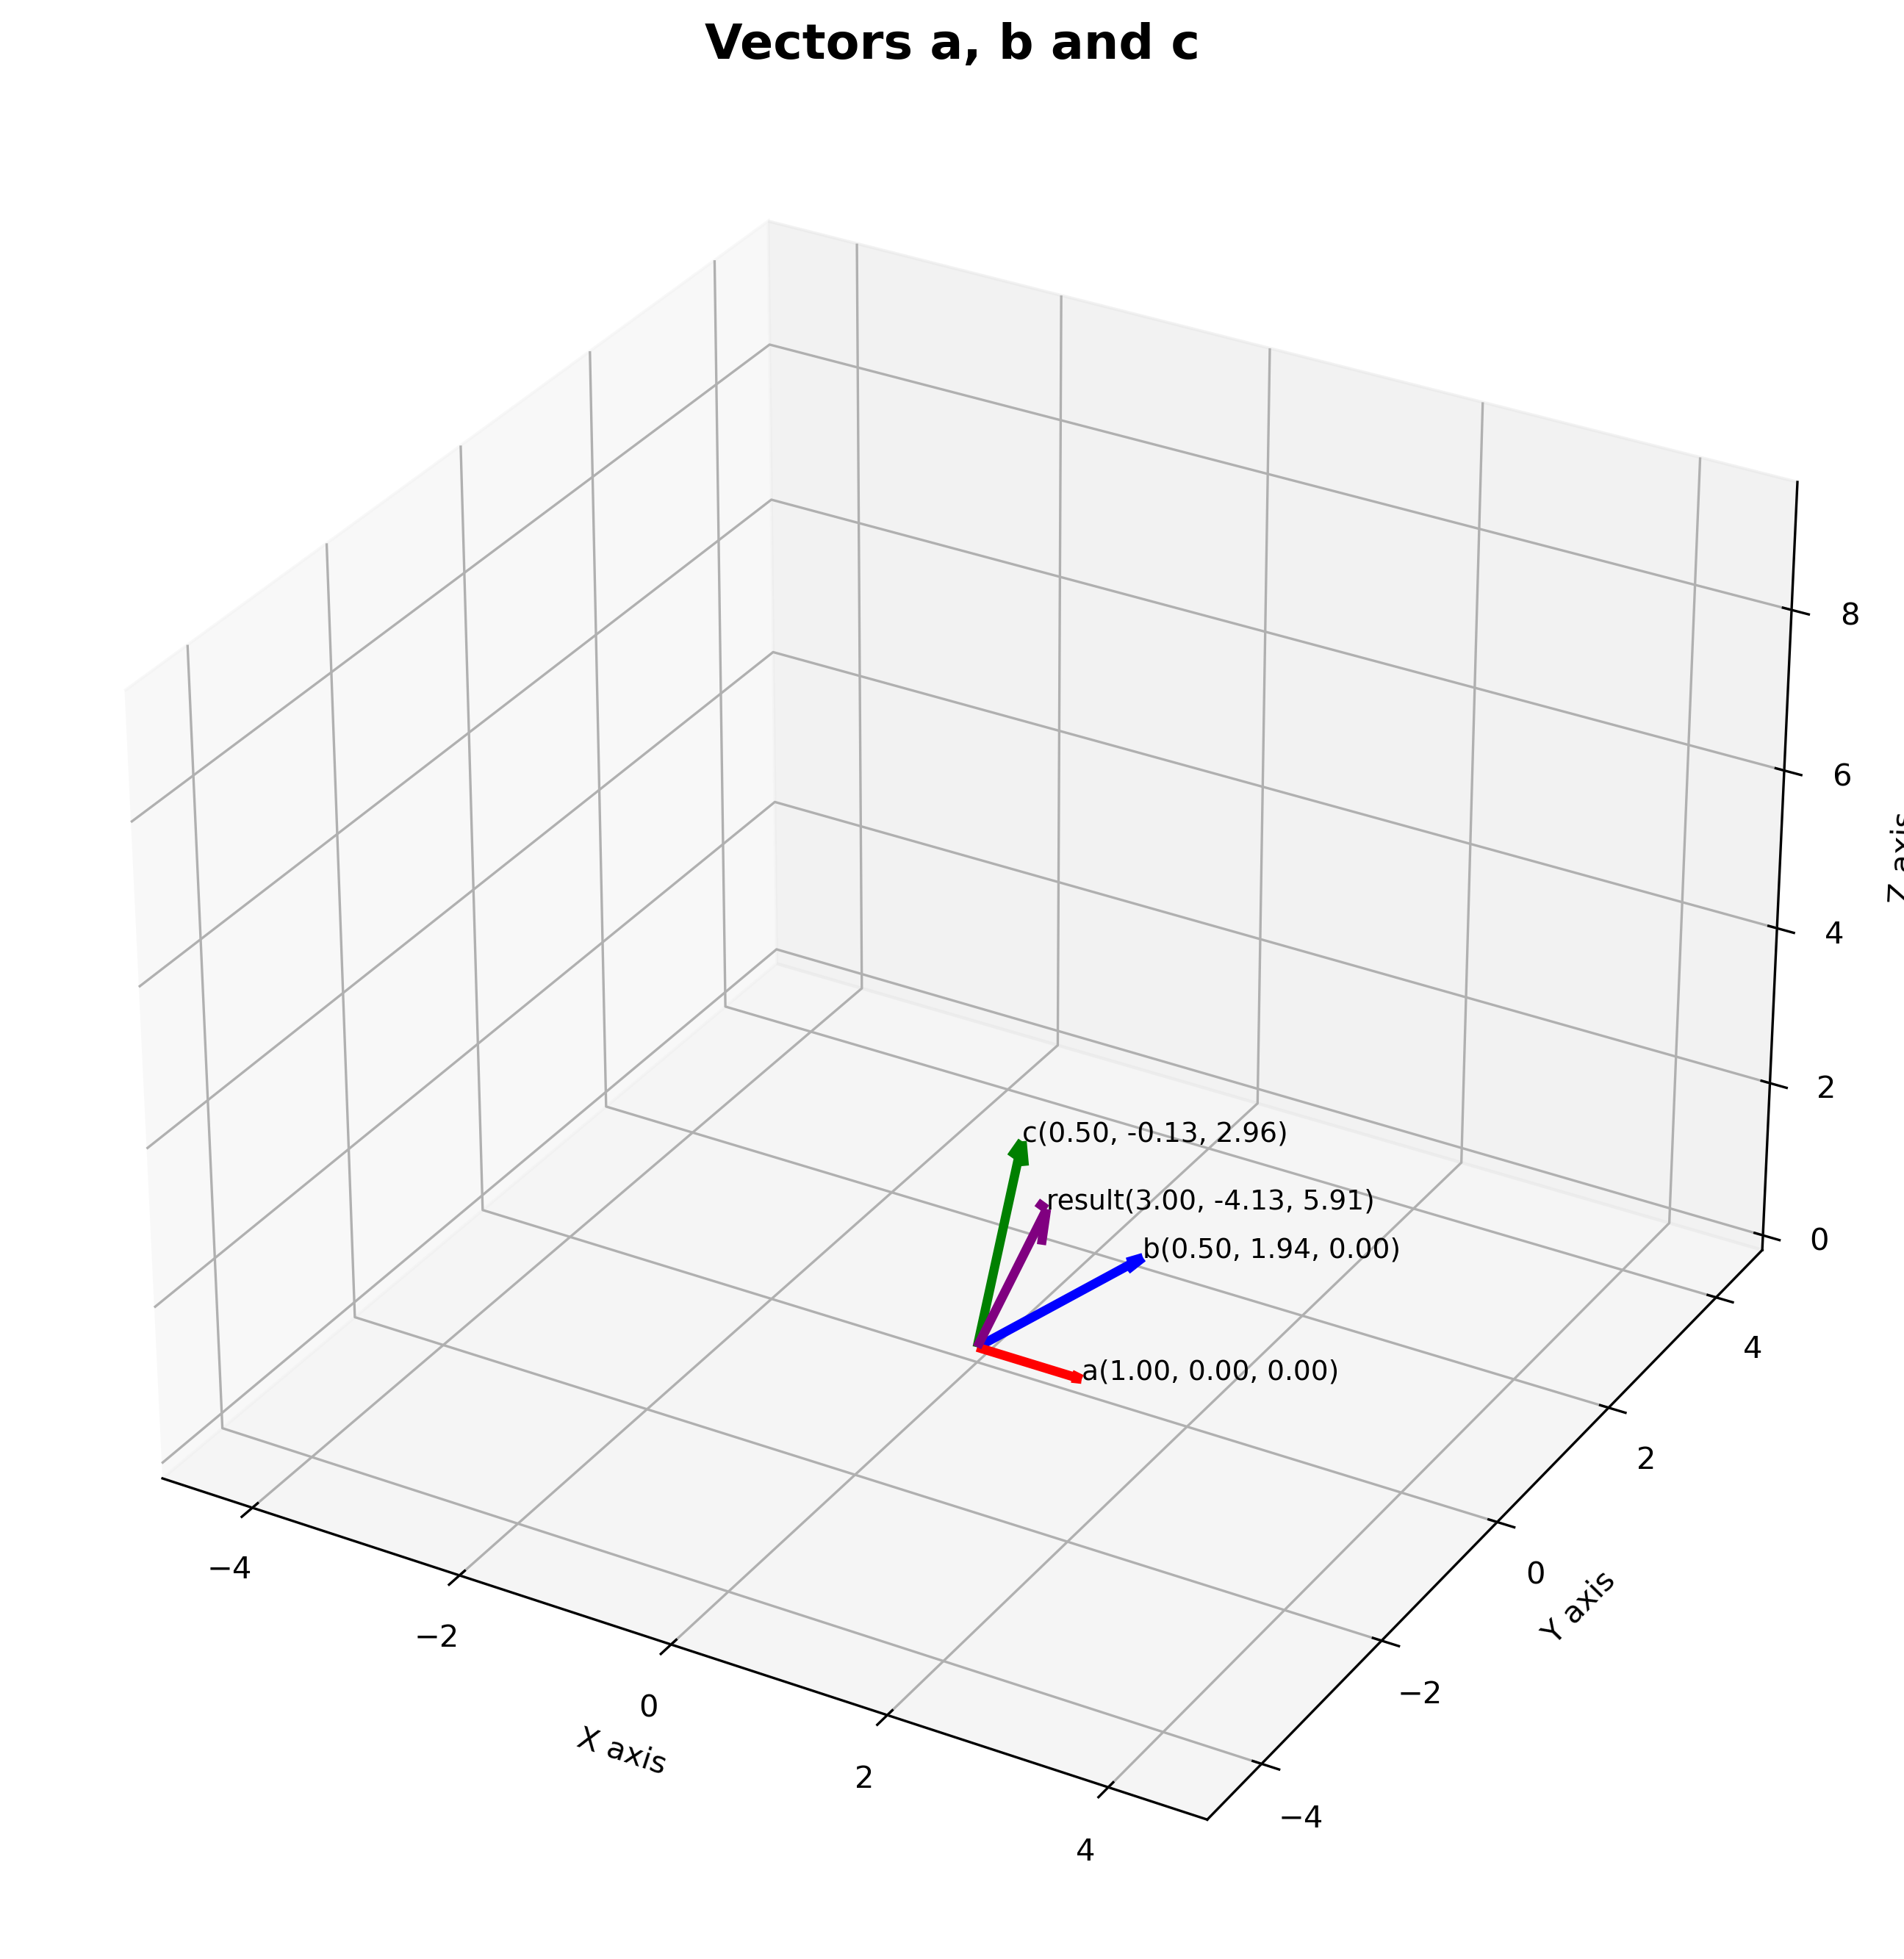
\includegraphics[width=\columnwidth]{figs/fig1.png}
    \caption{Vector Representation}
    \label{fig:fig/fig1.png}
\end{figure}
\end{document}  
